\documentclass[12pt]{article}

\usepackage[utf8]{inputenc}
\usepackage[T1]{fontenc}
\usepackage[ngerman]{babel}
\usepackage[ngerman=ngerman-x-latest]{hyphsubst}
\usepackage{csquotes}
\usepackage{hyphenat}
\usepackage{textcmds}
\usepackage{xspace}
\usepackage{listings}
\usepackage{amsmath}
\usepackage{amsfonts}
\usepackage{mathtools}
\usepackage{authblk}

\usepackage{geometry}
\geometry{a4paper, margin=1in}

\usepackage{graphicx}
\usepackage{chngpage}
\usepackage{calc}

\renewcommand{\lstlistingname}{Code}
\renewcommand{\lstlistlistingname}{Codeverzeichnis}

\usepackage{hyperref}
\hypersetup{
    colorlinks=true,
    linkcolor=black,
    filecolor=blue,
    urlcolor=blue,
    pdftitle={DBI Aufgabenblatt 5},
    pdfauthor={Nik Benson},
    pdfpagemode=FullScreen,
}
\urlstyle{same}

\usepackage{pgfplots}
\usepackage{pgfplotstable}

\usepackage{booktabs}
\usepackage{siunitx}
\usepackage{csvsimple}

\usepgfplotslibrary{units}

\usepackage{xcolor}
\definecolor{codegreen}{rgb}{0,0.6,0}
\definecolor{codegray}{rgb}{0.5,0.5,0.5}
\definecolor{codepurple}{rgb}{0.58,0,0.82}
\definecolor{backcolour}{rgb}{0.95,0.95,0.92}

\lstdefinestyle{java}{
    backgroundcolor=\color{backcolour},
    commentstyle=\color{codegreen},
    keywordstyle=\color{orange},
    numberstyle=\tiny\color{codegray},
    stringstyle=\color{codepurple},
    basicstyle=\ttfamily\footnotesize,
    breakatwhitespace=false,
    breaklines=true,
    captionpos=b,
    keepspaces=true,
    numbers=left,
    numbersep=5pt,
    showspaces=false,
    showstringspaces=false,
    showtabs=false,
    tabsize=2,
}

\lstset{style=java}

\DeclarePairedDelimiter\ceil{\lceil}{\rceil}
\DeclarePairedDelimiter\floor{\lfloor}{\rfloor}

\title{Praktikumsaufgabe 8 / 9 \\
\large Benchmark Datenbank - MySQL}
\author{Nik Benson, Luis Honderboom, Istvan Kovacs und Christopher Nattefort}


\usepackage[backend=biber,style=iso-authoryear]{biblatex}
\bibliography{sheet5}

\begin{document}
    \pagenumbering{gobble}
    \begin{titlepage}
    \clearpage
    \maketitle
    \vspace{2cm}
    \begin{center}
        
\includegraphics[width=\paperwidth/2]{assets/img/whs}
    \end{center}
    \vspace*{\fill}
    \begin{flushleft}
        \Large{\textbf{Institution:} Westfälische Hochschule}\\
        \Large{\textbf{Modul:} Datenbanken und Informationssysteme} \\
        \Large{\textbf{Prüfer:} Prof. Convent}\\
        \Large{\textbf{Semester:} WiSe 22/23}
    \end{flushleft}
\end{titlepage}


    \pagenumbering{Roman}
    \setcounter{page}{2}
    \addcontentsline{toc}{section}{Inhaltsverzeichnis}
    \tableofcontents
    \newpage
    \addcontentsline{toc}{section}{Abbildungsverzeichnis}
    \listoffigures
    \addcontentsline{toc}{section}{Tabellenverzeichnis}
    \listoftables
    \newpage
    \pagenumbering{arabic}

    \section{Einleitung}\label{sec:einleitung}
        \subsection{Aufgabenstellung}\label{subsec:aufgabenstellung}
Die vorgegebene Aufgabenstellung 8/9 im Praktikum von Datenbanken und Informationssysteme sieht eine Erstellung und Optimierung eines Java Programms, sowie eines Datenbankmanagementsystem vor.
Hierbei wurde in der vorherigen Aufgabe eine MySQL-Datenbank für die Dateninitialisierung in einer n-tps-Datenbank herangezogen, in der verschiedene Relationen erstellt und anschließend mit Einträgen bzw. Tupeln gefüllt wurden.
Bei dieser Aufgabenstellung sollen nun die erstellten Einträge mittels drei Abfragen / Lasttransaktionen (TXs) in einer 100-tps-Datenbank gelesen und verändert werden.
Die Benchmark-Messungen der Anfragen auf das DBMS erfolgen bei unterschiedlichen Lasten mit verschiedenen Profilen, die durch ein Load-Driver-Programm durchgeführt werden, wobei es eine 4-minütige Einschwingphase, dann eine 5-minütige Messphase und am Ende eine 1-minütige Ausschwingphase gibt.
\subsection{Datenbankmanagementsystem}\label{subsec:datenbankmanagementsystem-einleitung}
Als Datenbankmanagementsystem wird ein MySQL Server mit der Version 8.0.30 verwendet.
Dieser läuft auf einer virtuellen Maschine, der als Server agiert und durch eine Netzwerkverbindung zum Programm Abfragen / Transaktionen erhält.
Zum lokalen Testen des Programms auf dem eigenen Rechner wird ein Docker-Container mit MySQL Server-Instanz genutzt.
\subsection{Schema / Aufbau der Datenbank}\label{subsec:schema/aufbau}
Das Datenbankschema umfasst vier Relationen.
Diese sind nachfolgend als Abbildung dargestellt, sowie deren Verbindungen durch Fremdschlüssel der jeweiligen Relationen miteinander.
\begin{figure}[h!]
    \center
    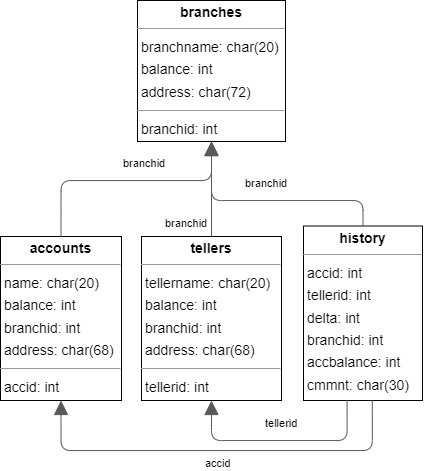
\includegraphics[height=8.5cm]{assets/img/benchmark-datenbank-schema}
    \caption{Benchmark-Datenbankschema}
    \label{fig:benchmark-datenbankschema}
\end{figure}
\subsection{Programme}\label{subsec:programme}
Verwendete Programme bei dieser Aufgabenstellung bezüglich der Erstellung und Optimierung des Java Programms und des Datenbankmanagementsystems sind unter anderen IntelliJ IDEA, MySQL Workbench CE, Data Grip, Docker, sowie der JDBC Treiber (Ver. 8.0.31) für die Schnittstelle/Kommunikation zwischen dem DBMS und dem Java Programm.
\subsection{Lasttransaktionen}\label{subsec:lasttransaktionen}
Nachfolgend werden die drei Abfragen / Lasttransaktionen (TXs) im Detail beschrieben.
Diese garantieren die bekannten ACID-Eigenschaften und werden nach einer relativen Gewichtung von 35 zu 50 zu 15 für Kontostand-, Einzahlungs- und Analyse-TX im Load-Driver-Programm ausgeführt.
\begin{enumerate}
    \item \textbf{Kontostands-TX} \\
    Eine Methode, die einen Kontostand (balance) zu der zugehörigen Kontonummer (accid) abfragt und als Rückgabewert liefert.
    \item \textbf{Einzahlungs-TX} \\
    Eine Methode / Abfrage, die als Einzahlung eines Betrages agiert und eine Kontonummer (accid), Geldautomatennummer (tellerid), Zweigstellennummer (branchid) und eine Einzahlungsbetrag (delta) als Eingabeparamter erwartet.
    In dieser Transaktion werden Einzelaktionen durchgeführt, wie das Aktualisieren der Bilanzsumme (balance) zu der zugehörigen Nummern (accid, branchid, tellerid) in den verschiedenen Relationen (accounts, branches, tellers).
    Des Weiterem das Erstellen einer Einzahlung als Beleg in der Relation history mit den zugehörigen Nummern (accid, branchid, tellerid), den Einzahlungsbetrag (delta), den aktualisierten Betrag (accbalance) von der Relation accounts, sowie einen Kommentar (cmmnt).
    Als Rückgabewert wird der aktualisierte Betrag (accblance) von der Relation accounts zurückgeben.
    \item \textbf{Analyse-TX} \\
    Eine Methode / Abfrage zur Ausgabe der Anzahl der getätigten Einzahlugen mit genau einem Betrags (delta), der als Eingabeparameter übergeben wird und diese als Rückgabewert zurückgibt.
\end{enumerate}


    \newpage

    \section{Dokumentation}\label{sec:dokumentation}
    \subsection{Version1}\label{subsec:version1}
\lstinputlisting[breaklines,language=Java,label={lst:version1-getBalanceFromAccount},caption={Quellcode zur Kontostandstransaktion der ersten Version}]{assets/code/version1/getBalanceFromAccount.java}
\lstinputlisting[breaklines,language=Java,label={lst:version1-updateBalance},caption={Quellcode zur Einzahlungstransaktion der ersten Version}]{assets/code/version1/getNumberOfDeltaBalance.java}
\lstinputlisting[breaklines,language=Java,label={lst:version1-getNumberOfDeltaBalance},caption={Quellcode zur Analysetransaktion der ersten Version}]{assets/code/version1/getNumberOfDeltaBalance.java}

\subsection{Version2}\label{subsec:version2}
\lstinputlisting[breaklines,language=Java,label={lst:version2-getBalanceFromAccount},caption={Quellcode zur Kontostandstransaktion der zweiten Version}]{assets/code/version2/getBalanceFromAccount.java}
\lstinputlisting[breaklines,language=Java,label={lst:version2-getNumberOfDeltaBalance},caption={Quellcode zur Analysetransaktion der zweiten Version}]{assets/code/version2/getNumberOfDeltaBalance.java}

\subsection{Version3 - Final}\label{subsec:version3---final}

    \newpage

    \section{Messungen}\label{sec:messungen}
    \subsection{Maximaler erreichbarer Transaktionsdurchsatz}\label{subsec:maximaler-erreichbarer-transaktionsdurchsatz}
Um den maximalen erreichbaren Transaktionsdurchsatz zu berechnen, müssen nur die begrenzenden Variablen, in diesem Fall Think-Time mit 50 ms, angeschaut werden.
Infolgedessen wird theoretisch angenommen, dass die verschiedenen Lasttransaktionen bei der Ausführung keine Zeit beanspruchen.
Schließlich ergibt sich dann aus dem Messzeitraum von 300s (5 min) und der begrenzenden Variable mit 0,05s der maximale erreichbare Transaktionsdurchsatz pro Thread im Loaddriver von 6.000 TXs (300s / 0,05s) und somit 20 TXs pro Sekunde.
Außerdem kann aus der relativen Gewichtung für die unterschiedlichen Lasttransaktionen folgende Verteilung der Transaktionsanzahl der verschiedenen Lasttransaktionen und Last-Profilen bestimmt werden.
\begin{table}[h!]
    \centering
    \begin{tabular}{|c|c|c|}
        \hline
        Lasttransaktion & relative Gewichtung [\%] & Transaktionsanzahl [TXs] \\  \hline
        Kontostands-TX & 35 & 2.100 \\ \hline
        Einzahlungs-TX & 50 & 3.000 \\ \hline
        Analyse-TX & 15 & 900 \\ \hline
    \end{tabular}
    \caption{Tabelle für die Verteilung der Transaktionsanzahl der unterschiedlichen Lasttransaktionen bei verschiedenen relativen Gewichtungen}
    \label{tab:1}
\end{table}
\begin{table}[h!]
    \centering
    \begin{tabular}{|c|l|c|}
        \hline
        Last & Berechnung [\%] & Transaktionsdurchsatz [TXs/s] \\  \hline
        Last1 & 5 x Threads * 20 TXs/s & 100 \\ \hline
        Last2 & 2 x Client (5 x Threads * 20 TXs/s) & 200 \\ \hline
        Last3 & 3 x Client (5 x Threads * 20 TXs/s) & 300 \\ \hline
    \end{tabular}
    \caption{Tabelle für den Transaktiondurchsatz pro Sekunde bei den verschiedenen Last-Profilen}
    \label{tab:2}
\end{table}

\subsection{Last1: Benchmark für 5 remote Load Driver}\label{subsec:benchmark-5-remote-load-driver}
\begin{table}[h!]
    \centering
    \begin{tabular}{|c|c|c|c|c|c|}
        \hline
        Version & Gesamte TXs & Kontostands-TXs & Analyse-TXs & Einzahlungs-TXs & TXs \\  \hline
        1 & 20.718 & 2.021 & 386 & 217 & 69 \\ \hline
        2 & 20.740 & 1.763 & 381 & 219 & 69 \\ \hline
        3 & 20.785 & 1.731 & 376 & 214 & 69 \\ \hline
        4 & - & - & - & - & - \\ \hline
        5 & - & - & - & - & - \\ \hline
    \end{tabular}
    \caption{Messergebnisse des Benchmarks bei Last1 (Transaktionen pro Sekunde)}
    \label{tab:3}
\end{table}

\newpage

\subsection{Last2: Benchmark für 5+5 remote Load Driver}\label{subsec:benchmark-5-5-remote-load-driver}
\begin{table}[h]
    \centering
    \begin{tabular}{|c|c|c|c|c|c|}
        \hline
        Version & Gesamte TXs & Kontostands-TXs & Analyse-TXs  & Einzahlungs-TXs & TXs \\  \hline
        1 & 39.737 & 2.545 & 412 & 418 & 132 \\ \hline
        2 & 39.777 & 2.524 & 407 & 413 & 133 \\ \hline
        3 & 39.912 & 2.614 & 414 & 420 & 133 \\ \hline
        4 & 42.694 & 4.355 & 4.780 & 469 & 142 \\ \hline
        5 & 42.835 & 4.333 & 4.773 & 498 & 143 \\ \hline
    \end{tabular}
    \caption{Messergebnisse des Benchmarks bei Last2 (Transaktionen pro Sekunde)}
    \label{tab:4}
\end{table}

\subsection{Last3: Benchmark für 5+5+5 remote Load Driver}\label{subsec:benchmark-5-5-5-remote-load-driver}
\begin{table}[h]
    \centering
        \begin{tabular}{|c|c|c|c|c|c|}
            \hline
            Version & Gesamte TXs & Kontostands-TXs & Analyse-TXs  & Einzahlungs-TXs & TXs \\  \hlinen
            1 & 51.080 & 2.644 & 505 & 326 & 170 \\ \hline
            2 & 54.824 & 2.103 & 438 & 468 & 183 \\ \hline
            3 & 54.754 & 2.152 & 435 & 467 & 182 \\ \hline
            4 & 63.997 & 6.514 & 7.197 & 735 & 213 \\ \hline
            5 & 64.299 & 6.492 & 7.229 & 764 & 228 \\ \hline

        \end{tabular}
        \caption{Messergebnisse des Benchmarks bei Last3 (Transaktionen pro Sekunde)}
        \label{tab:5}
\end{table}

    \newpage

    \section{Optimierungen}\label{sec:optimierungen}
        [Einleitung]
\subsection{Verbesserungsideen}\label{subsec:verbesserungsideen}

\subsection{Programmcode}\label{subsec:programmcode}

\subsection{Datenbankmanagementsystem}\label{subsec:datenbankmanagementsystem}

    \newpage

    \section{Fazit}\label{sec:fazit}
        Zusammenfassend kann man sagen, dass die vorgenommenen Optimierungen im Hinblick auf einen performanteren Code die Laufzeit deutlich verbessert haben.\\
\\
Denn bei der ersten Version unseres Programms wurde eine schlechte Laufzeit für nur n = 1 (100.000 Tupel in Accounts) mit 466 Sekunden remote gemessen.
Wohingegen schon bessere Laufzeiten aufgrund der ersten Optimierung am Code durch das Bündeln der Statements in einzelne Batches erreicht werden konnte.
Dennoch konnte man keine Konsistenz in den Messwerten bei den Batches sehen, woraufhin wir eine andere Optimierungsmöglichkeit in Betracht gezogen haben.
Diese wäre das asynchrone Ausführen von INSERT\-Statements mit vielen Tupeln in mehreren Threads.
Durch diese Optimierung konnte eine deutliche Verbesserung der Laufzeit erzielt werden, da für n = 10 (1.000.000 Tupel in Accounts) nur eine Laufzeit von 32 Sekunden gemessen wurde.\\
\\
Bei den Optimierungen der Datenbankmanagementsystem\-Konfigurationen konnten keine signifikanten Verbesserungen für ein performanteres DBMS erreicht werden.
Dementgegen wurden eher Verschlechterungen der Laufzeit gemessen.

    \newpage
    \pagenumbering{roman}
    \printbibliography

    \section{Anhang}\label{sec:anhang}
        \subsection*{Programmcode}\label{subsec:programmcode-anhang}
\lstinputlisting[breaklines,language=Java,label={lst:anhand-loadriver},caption={Quellcode zur Loaddriver-Klasse}]{assets/code/loadDriver.java}
\subsubsection*{Version1}
\lstinputlisting[breaklines,language=Java,label={lst:anhand-ntpsDatenbankTransaktion-version1},caption={Quellcode zur NTPSDatenbankTransaktions-Klasse der ersten Version}]{assets/code/version1/ntpsDatenbankTransaktion.java}
\subsubsection*{Version2}
\lstinputlisting[breaklines,language=Java,label={lst:anhand-ntpsDatenbankTransaktion-version2},caption={Quellcode zur NTPSDatenbankTransaktions-Klasse der zweiten Version}]{assets/code/version2/ntpsDatenbankTransaktion.java}
\subsubsection*{Version3}
\lstinputlisting[breaklines,language=Java,label={lst:anhand-ntpsDatenbankTransaktion-version3},caption={Quellcode zur NTPSDatenbankTransaktions-Klasse der dritten Version}]{assets/code/version3/ntpsDatenbankTransaktion.java}
\subsubsection*{Version5}
\lstinputlisting[breaklines,language=Java,label={lst:anhand-ntpsDatenbankTransaktion-version5},caption={Quellcode zur NTPSDatenbankTransaktions-Klasse der fünften Version}]{assets/code/version5/ntpsDatenbankTransaktion.java}
\end{document}
